The sensitivity of the search on the resonant is expected to increase by distinguishing the type of parton that initiated the jets. The parton types of dijet events as a function of \mjj from the MC with a  \textsc{Pythia8.186} at LO  NNPDF2.3 PDFs is shown in Figure~\ref{fig:quarkgluonfraction}, suggesting that the search for new resonance can be improved by tagging quark and gluon jets.

%ATLAS has published a study \cite{ATL-PHYS-PUB-2017-009} 

In this section we present the search for new particles using the full Run~2 $\sqrt{s} = 13$~TeV\xspace dataset with quark and gluon tagging method.


\begin{figure}[htb]
 \centering
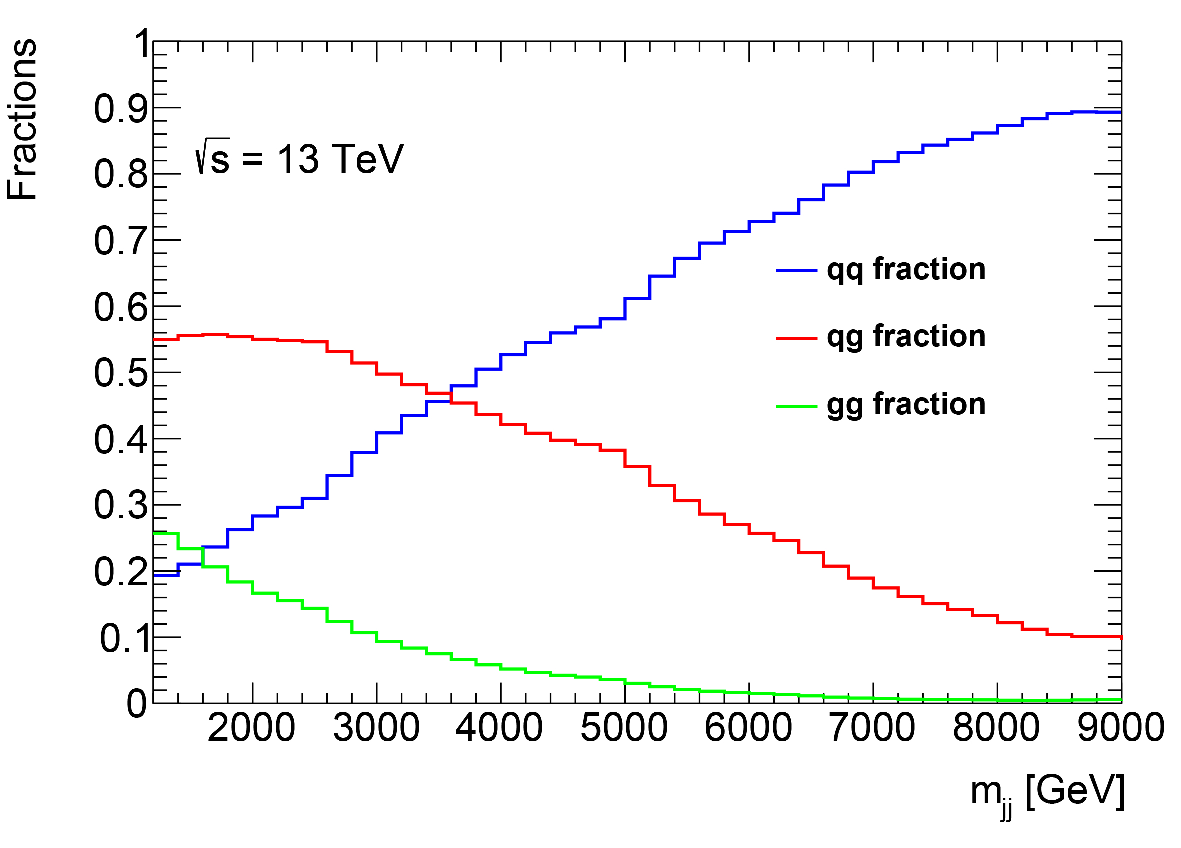
\includegraphics[width=0.75\textwidth]{fig/tagging/Fractions_QCD.pdf}
\caption{The fraction of dijet events that are initiated by quark-quark events (blue), quark-gluon 
events (green) and gluon-gluon events (red) in simulated data.  \label{fig:quarkgluonfraction}}
\end{figure}


Previous study in ATLAS has shown that the jets can be tagged quark or gluon jets based on the number of charged tracks associated with the jets with \pt~above 500 MeV. Samples with enhanced fractions of quark or gluon initiated jets can be created by using a selection based on the charged-particle constituent multiplicity \ntrk. As shown in Fig.~\ref{fig:jet_pt_quark_gluon}, where \pythia8 generator~is used for MC to ensure a good agreement with the distribution of \ntrk~in data within the ID acceptance $|\eta|<2.1$.

\begin{figure}[htb]
 \centering
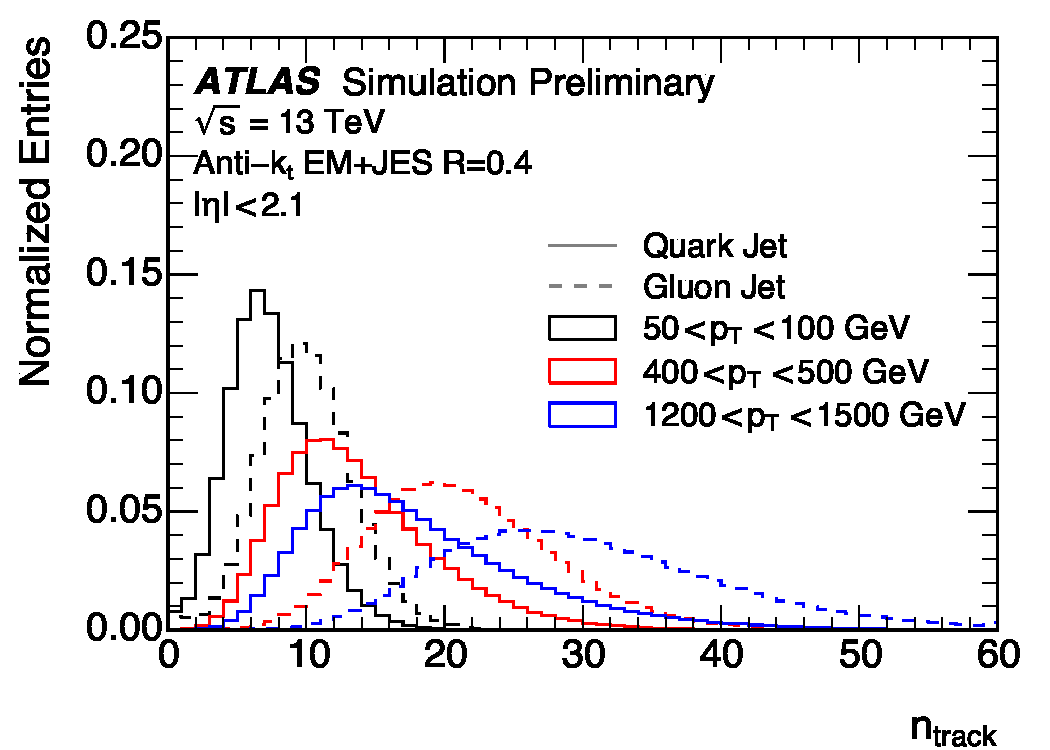
\includegraphics[width=0.65\textwidth]{fig/tagging/fig_01_ATL-PHYS-PUB-2017-009.pdf}
\caption{Distribution of the jet reconstructed track multiplicity (\ntrk ) in
 different \pt\ ranges with the \pythia~8 MC samples and processes with a full simulation of the
 ATLAS detector. Tracks are required to have $\pt~> 500$ MeV and pass
  quality criteria described in Ref.~\cite{ATL-PHYS-PUB-2017-009}. }
\end{figure}


\subsubsection{Expected Signal Significance}
%\label{sec:ExpectedSig}

The shape of \mjj from QCD is complex and rapidly changing according to the fractions of events that originate from quark-quark, quark-gluon and gluon-gluon scattering. The QCD background is presented in Section~\ref{qcdsamps}. The MC simulated signals and background is thus used for estimating the expected signal significance.


\paragraph{Resonances that decay to quark-quark\\}

The statistical significance associated with signals decaying into quark-antiquark pairs is assessed using \Zprime\ models using 
\begin{equation}
	S = N_S \sum_i{ \dfrac{ f_{qq,i}\epsilon_{qQ}^2 + f_{qg,i}\epsilon_{qQ}\epsilon_{gQ} + f_{gg.i}\epsilon_{gQ}^2  } {\sqrt{ B_{qq,i}\epsilon_{qQ}^2 + B_{qg,i}\epsilon_{qQ}\epsilon_{gQ} + B_{gg,i}\epsilon_{gQ}^2  }}}
\end{equation}
where $N_S$ is the number of signal events, $f_{qq,i}$ is fraction of signal events that result in the two 
highest \pT\ jets that where initiated by quarks in bin $i$ ( $f_{qg,i}$ are quark-gluon jets, and $f_{gg,i}$ is two gluon jets), 
$\epsilon_{qQ}$ is the efficiency of a quark initiated jet passing the quark selection criteria, 
$\epsilon_{gQ}$ is the efficiency of a gluon initiated jet passing the quark selection criteria, 
and $B_{xx,i}$ is the expected number of background events with quark-quark, quark-gluon or gluon-gluon initiated jets. 


The statistical significance is computed for \Zprime\ particles mass values within the range of 1500 to 4000 GeV, and for quark-jet selection efficiencies ranging from 30\% to 90\%. The obtained significance values are presented in Figure~\ref{fig:QuarkSignalSignificance}. The depicted results illustrate a trend of diminishing significance when any quark-selection criteria is imposed on the data. This decline in significance can be attributed to the dominant presence of quark-quark events within the data, where the selection process concurrently diminishes both background and signal contributions to a comparable extent.

\begin{figure}[htb]
	\centering
	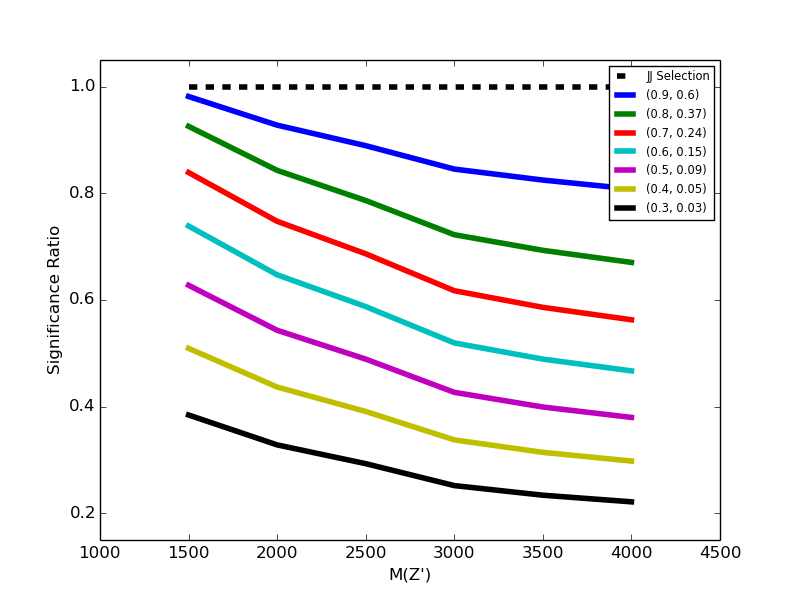
\includegraphics[width=0.75\textwidth]{fig/tagging/QuarkSignalSignificance.png}
	\caption{ The significance for observing a \Zprime\ with masses from 1500 to 4000 GeV
		for $\epsilon_{qQ}$ ranging from 90 to 30\% compared to the significance calculated with no quark selection applied. The key gives pairs of efficiencies ($\epsilon_{qQ}$, $\epsilon_{gQ}$).
		\label{fig:QuarkSignalSignificance}}
\end{figure}


\paragraph{Signals that decay to gluon-gluon\\}
The significance for signals that decay to a gluon-gluon pair are using \Hprime\ models, estimated by:
\begin{equation}
S = N_S \sum_i{ \dfrac{ f_{qq,_i}\epsilon_{qG}^2 + f_{qg,i}\epsilon_{qG}\epsilon_{gG} + f_{gg,i}\epsilon_{gG}^2  } {\sqrt{ B_{qq,i}\epsilon_{qG}^2 + B_{qg,i}\epsilon_{qG}\epsilon_{gG} + B_{gg,i}\epsilon_{gG}^2  }}}
\end{equation}
where  
$\epsilon_{qG}$ is the efficiency of a quark initiated jet passing the gluon selection criteria, 
$\epsilon_{gG}$ is the efficiency of a gluon initiated jet passing the gluon selection criteria. 

The computation of significance involves the utilization of simulated \Hprime signals, with masses ranging from 2000 to 7000 GeV. The efficiencies of gluon tagged are varied across from 60\% to 90\%. The resulting significances, depicted as functions of \Hprime masses, are presented in Figure~\ref{fig:GluonSignalSignificance}. The observed trend reveals a gradual increase in significance, with values ascending from approximately 1.2 at 2 TeV to around 1.6 at 7 TeV. Notably, the most substantial enhancements occur at a gluon efficiency of 75\%.


\begin{figure}[htb]
 \centering
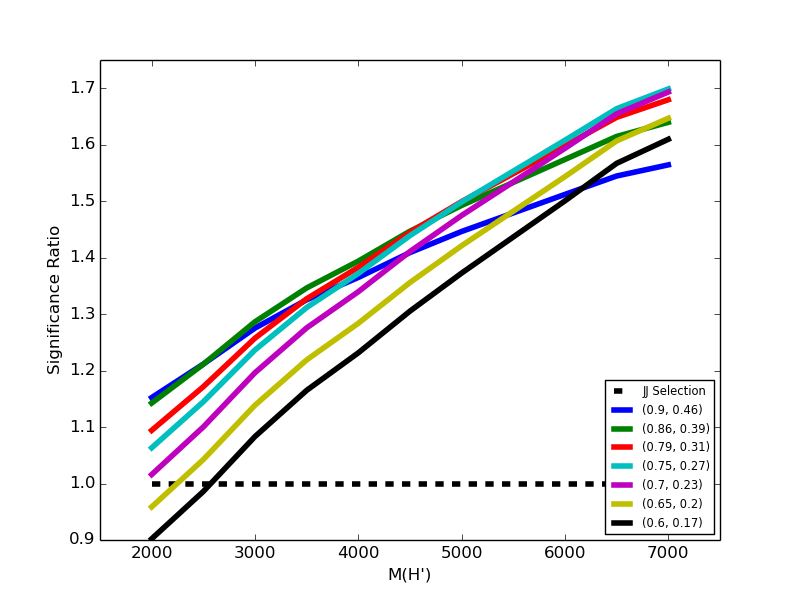
\includegraphics[width=0.75\textwidth]{fig/tagging/GluonSignalSignificance.png}
\caption{ The significance for observing a \Hprime\ with masses from 2000 to 7000 GeV
for $\epsilon_{gG}$ ranging from 90 to 60\% compared to the significance calculated with no gluon selection applied. The key gives pairs of efficiencies ($\epsilon_{gG}$, $\epsilon_{qG}$).
  \label{fig:GluonSignalSignificance}}
\end{figure}


\paragraph{Signals that decay to quark-gluon\\}

Calculating the significance for signals involving quark-gluon decays, such as string decays, poses increased complexity due to the potential overlap in the selection criteria between decaying jets that satisfy both quark and gluon criteria. In this context, it becomes imperative to establish distinct efficiencies exclusively tailored for quark- and gluon-jets. Thus the efficiencies are needed to be defined exclusively for quark- and gluon-jets.

The efficiencies for quark-jets are defined as:

\begin{itemize}
\item $\epsilon_{qQ}$ The efficiency that a quark-jet is identified only as a quark-jet. 
\item $\epsilon_{qQG}$ The efficiency that a quark-jet is identified as a quark- and a gluon-jet.
\item $\epsilon_{qG}$ The efficiency that a quark-jet is identified only as a gluon-jet.  
\end{itemize}
where $\epsilon_{qQ} + \epsilon_{qQG} + \epsilon_{qG} = 1$. 

Another set of efficiencies that is measured for gluon-jets are:
\begin{itemize}
\item $\epsilon_{gQ}$ The efficiency that a gluon-jet is identified only as a quark-jet. 
\item $\epsilon_{gQG}$ The efficiency that a gluon-jet is identified  as a quark- and a gluon-jet.
\item $\epsilon_{gG}$ The efficiency that a gluon-jet is identified only as a gluon-jet.  
\end{itemize}

The probability of truth pairs of quark-quark ($p_{qq}$), quark-gluon ($p_{qg}$) and gluon-gluon ($p_{gg}$) events that passing the quark-gluon tagging selection criteria are given by:
\begin{align}
p_{qq} & = 2  \epsilon_{qQ}\epsilon_{qG} + \epsilon_{qQG}\left( \epsilon_{qQ} + \epsilon_{qG} \right)  + \epsilon_{qQG}\epsilon_{qQG} \\
p_{gg} & = 2  \epsilon_{gQ}\epsilon_{gG} + \epsilon_{gQG}\left( \epsilon_{gQ} + \epsilon_{gG} \right)  + \epsilon_{gQG}\epsilon_{gQG} \\
p_{qg} & = \epsilon_{qQ}\epsilon_{gG} + \epsilon_{gQ}\epsilon_{qG} + \epsilon_{qQG}\left( \epsilon_{gQ} + \epsilon_{gG} \right) 
+ \epsilon_{gQG}\left( \epsilon_{qQ} + \epsilon_{qG} \right) 
+ \epsilon_{gQG}\epsilon_{gQG}
\end{align}
the related significance is then defined as:
\begin{equation}
S = N_S \sum_i{ \dfrac{ f_{qq,i} p_{qq} + f_{qg,i}p_{qg} + f_{gg,i}p_{gg}  } {\sqrt{ B_{qq,i}p_{qq} + B_{qg,i}p_{qg} + B_{gg,i}p_{gg}  }}}.
\end{equation}

No obvious benefit is observed after applied a quark selection with selection efficiencies from 30 to 100\%. A small but significant improvement is obtained in significance by applying a gluon selection to one of the two leading jets.
The resulting significances are  in Fig.~\ref{fig:QuarkGluonSignalSignificance} where an increase of 25\% in significance at masses above 5 TeV is obtained, with the largest increases happening over 70\% gluon efficiency.

\begin{figure}[htb]
 \centering
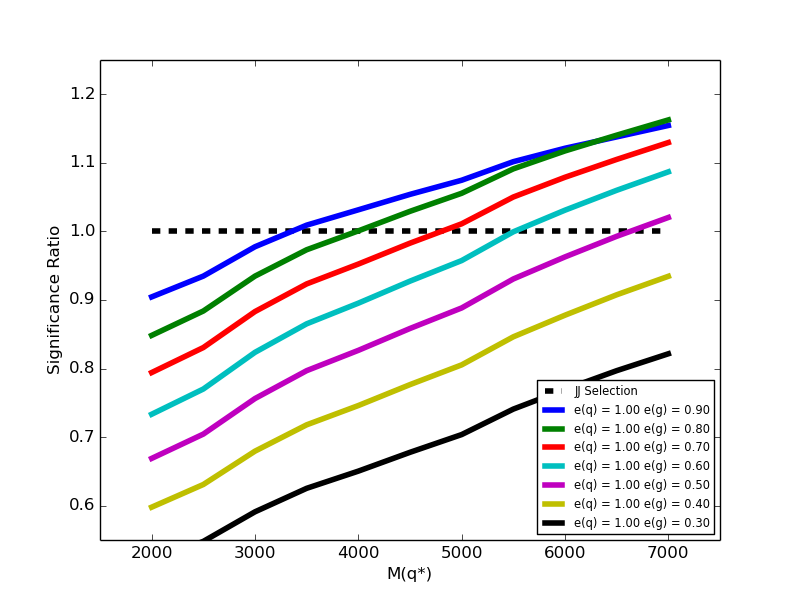
\includegraphics[width=0.75\textwidth]{fig/tagging/QuarkGluonSignalSignificance3.png}
\caption{ The significance for observing a \qstar\ with masses from 2000 to 7000 GeV 
for $\epsilon_{gG}$ ranging from 30 to 90\% compared to the significance calculated with no gluon selection applied. The key gives pairs of efficiencies ($\epsilon_{gG}$, $\epsilon_{qG}$).
  \label{fig:QuarkGluonSignalSignificance}}
\end{figure}

\FloatBarrier

\subsubsection{Selection Criteria}

The selection criteria for an quark-enriched jet sample was chosen so that 60\% quark-initiated purity is achieved in each jet \pt~bin. However, discontinuities in the \mjj spectrum would occur when such criteria is applied to the high mass (\pt~> 5000 GeV), leads to difficulties presented in resonance search. 


A selection criteria is thus built as a linear function of the $\ln(\pt) $, results in a smooth \mjj distribution. A jet is tagged as being more likely to be quark-initiated if \ntrk~is less than
the threshold \nq and more likely to be gluon-initiated if \ntrk~is 
greater than the threshold \ngluon: 
\begin{align}
\ntrk & \le \nq \; \mbox{quark-initiated sample} %\label{eq:QGselect}  % uncomment if label used. 
\\
\ntrk	  & \ge \ngluon \; \mbox{gluon-initiated sample} \nonumber
\end{align}
where   
\begin{equation}
n_{\mathrm{q(g)}} = {c_{\mathrm{q(g)}} + m_{\mathrm{q(g)}} \ln(\pt)}  \label{eq:nqg2}
\end{equation}
parameters $m_{\mathrm{q(g)}}$ and $c_{\mathrm{q(g)}}$ are constants obtained from the MC samples, these are founded by  finding the value of \ntrk\ 
that corresponds to a given efficiency for truth quark and gluon jets in 
\pt~bins, and chosen to defined suitable subsamples, the \pt~here is in units of GeV.

For each \pt~bin, the number of tracks \ntrk\ that closest to the given selection efficiency is found. Because the \ntrk~is an integer number of track thus does not correspond exactly to the selection efficiency, a linear interpolation is carried out between the given efficiencies of the selected bin and the closest bin of it, to correct the  fractional number of tracks that corresponds to the selection efficiency, the corresponding uncertainty is evaluated as binomial distribution. 


The jet \pt~bin edges are divided into 
480, 500, 520, 540, 560, 580, 600, 625, 650, 700, 750, 800, 900, 1000, 1400, 
1600, 1800, 2000, 2500, 3000, 3500, 4000, 5000, 6000 GeV. An example of the cumulative 
distribution of \ntrk~for truth quark- and gluon-jets at the \pt~range of 800 - 900 GeV is shown in
Figure~\ref{fig:ntrk_cumulative_app}.


\begin{figure}[htb]
 \centering
\includegraphics[width=0.75\textwidth]{fig/tagging_variation/Cumulative_ntrk_distribution_12_800_900GeV.pdf}
\caption{The cumulative distribution of \ntrk\ for truth quark- (blue) and gluon- (red)jets 
satisfying 800 < \pt~< 900 GeV.  \label{fig:ntrk_cumulative_app}}
\end{figure}

The coefficients for Equation~\ref{eq:nqg2} are determined for quark and gluon selection efficiencies ranging from 65\% to 95\% in increments of 5\%. The plot showcasing the \ntrk\ values corresponding to selection efficiencies of 70\%, 75\%, and 80\% is depicted in Figure~\ref{fig:qg_selection_curves_app}, along with the optimal fit employing Equation~\ref{eq:nqg2}. The constants' values for both quark and gluon selections are summarized in Tables~\ref{table:truthQuarkSelectionEfficiencies_app} and \ref{table:truthGluonSelectionEfficiencies_app}. For a selection efficiency of 75\%, the fitting yields a $\chi^2$ of $33.5$ (quark selection) and $2.6$ (gluon selection) for 21 degrees of freedom.

Notably, the \ntrk\ value that satisfies the selection efficiency attains a plateau above 4000 GeV, suggesting the potential presence of a saturation effect. To validate these findings, the data is subjected to an alternative fit function. An alternative fit function is derived as a cross check: 

\begin{equation}
	n_{\mathrm{q(g)}} = {c + m \ln(\pt) + n \sqrt{\ln(\pt)}}. \label{eq:nqg3}
\end{equation}
which improve the $\chi^2$ of the fit in a selection efficiency of 75\% from $33.5$ to $25.1$ in quark-selection, and from $2.6$ to $1.6$ in gluon-selection.  Figure~\ref{fig:qg_selection_curves2} shows the alternative fit for quark and gluon selections. The values of the constants for both quark and gluon selections 
are summarised in Tables~\ref{table:truthQuarkSelectionEfficiencies2} and \ref{table:truthGluonSelectionEfficiencies2}. 



The values of the constants for both quark and gluon selections are summarised in 
Tables~\ref{table:truthQuarkSelectionEfficiencies_app} and \ref{table:truthGluonSelectionEfficiencies_app}. 
\begin{table}[h]
	\centering 
	
	\begin{tabular}{SSSS}
		\toprule
		\multicolumn{1}{c}{Truth-$q$ selection efficiency}   & \multicolumn{1}{c}{Truth-$g$ selection efficiency} &  \multicolumn{1}{c}{$c$}  &  \multicolumn{1}{c}{$m$} \\
		\midrule 
		0.95 & 0.732 & -27.568 & 8.789 \\
		0.90 & 0.563 & -21.518 & 7.269 \\
		0.85 & 0.447 & -17.646 & 6.304 \\
		0.80 & 0.350 & -14.956 & 5.610 \\
		0.75 & 0.278 & -12.600 & 5.022 \\
		0.70 & 0.221 & -10.691 & 4.536 \\
		0.65 & 0.174 & -8.990 & 4.105 \\
		\bottomrule
	\end{tabular}
	\caption{ Values of constants $m$ and $c$ from Equation.~\ref{eq:nqg2} such that $ \ntrk  \le \nq $ 
		for truth quark jets for a range of efficiencies  from 65 to 95\%. 
		\label{table:truthQuarkSelectionEfficiencies_app}
	}
\end{table}

\begin{table}[h]
	\centering 
	
	\begin{tabular}{SSSS}
		\toprule
		\multicolumn{1}{c}{Truth-$g$ selection efficiency}   & \multicolumn{1}{c}{Truth-$q$ selection efficiency} &  \multicolumn{1}{c}{$c$}  &  \multicolumn{1}{c}{$m$} \\
		\midrule 
		0.95 & 0.586 & -7.541 & 3.233 \\
		0.90 & 0.456 & -8.980 & 3.779 \\
		0.85 & 0.377 & -10.419 & 4.230 \\
		0.80 & 0.320 & -11.964 & 4.659 \\
		0.75 & 0.274 & -13.376 & 5.047 \\
		0.70 & 0.234 & -14.937 & 5.446 \\
		0.65 & 0.202 & -16.466 & 5.834 \\
		\bottomrule
	\end{tabular}
	\caption{ Values of constants $m$ and $c$ from Equation~\ref{eq:nqg2} such that $ \ntrk  \ge \ngluon $ 
		for truth quark jets for a range of efficiencies  from 65 to 95\%. 
		\label{table:truthGluonSelectionEfficiencies_app}
	}
\end{table}




\begin{table}[h]
	\centering 
	
	\begin{tabular}{SSSSS}
	\toprule
\multicolumn{1}{c}{Truth-$q$ selection efficiency}   & \multicolumn{1}{c}{Truth-$g$ selection efficiency} &  \multicolumn{1}{c}{$c$}  &  \multicolumn{1}{c}{$m$} &  \multicolumn{1}{c}{$n$} \\
\midrule 
0.80 & 0.350 & -139.822 & -11.714 & 93.100 \\
0.75 & 0.278 & -128.174 & -11.001 & 86.141 \\
0.70 & 0.221 & -128.255 & -11.755 & 87.604 \\
\bottomrule
\end{tabular}
	\caption{ Values of constants $m$ and $c$ from Equation~\ref{eq:nqg3} such that $ \ntrk  \le \nq $ 
	for truth quark jets for a range of efficiencies  from 70 to 80\%. 
	\label{table:truthQuarkSelectionEfficiencies2}
}
\end{table}

\begin{figure}[p]
	\centering
	\subfloat[] {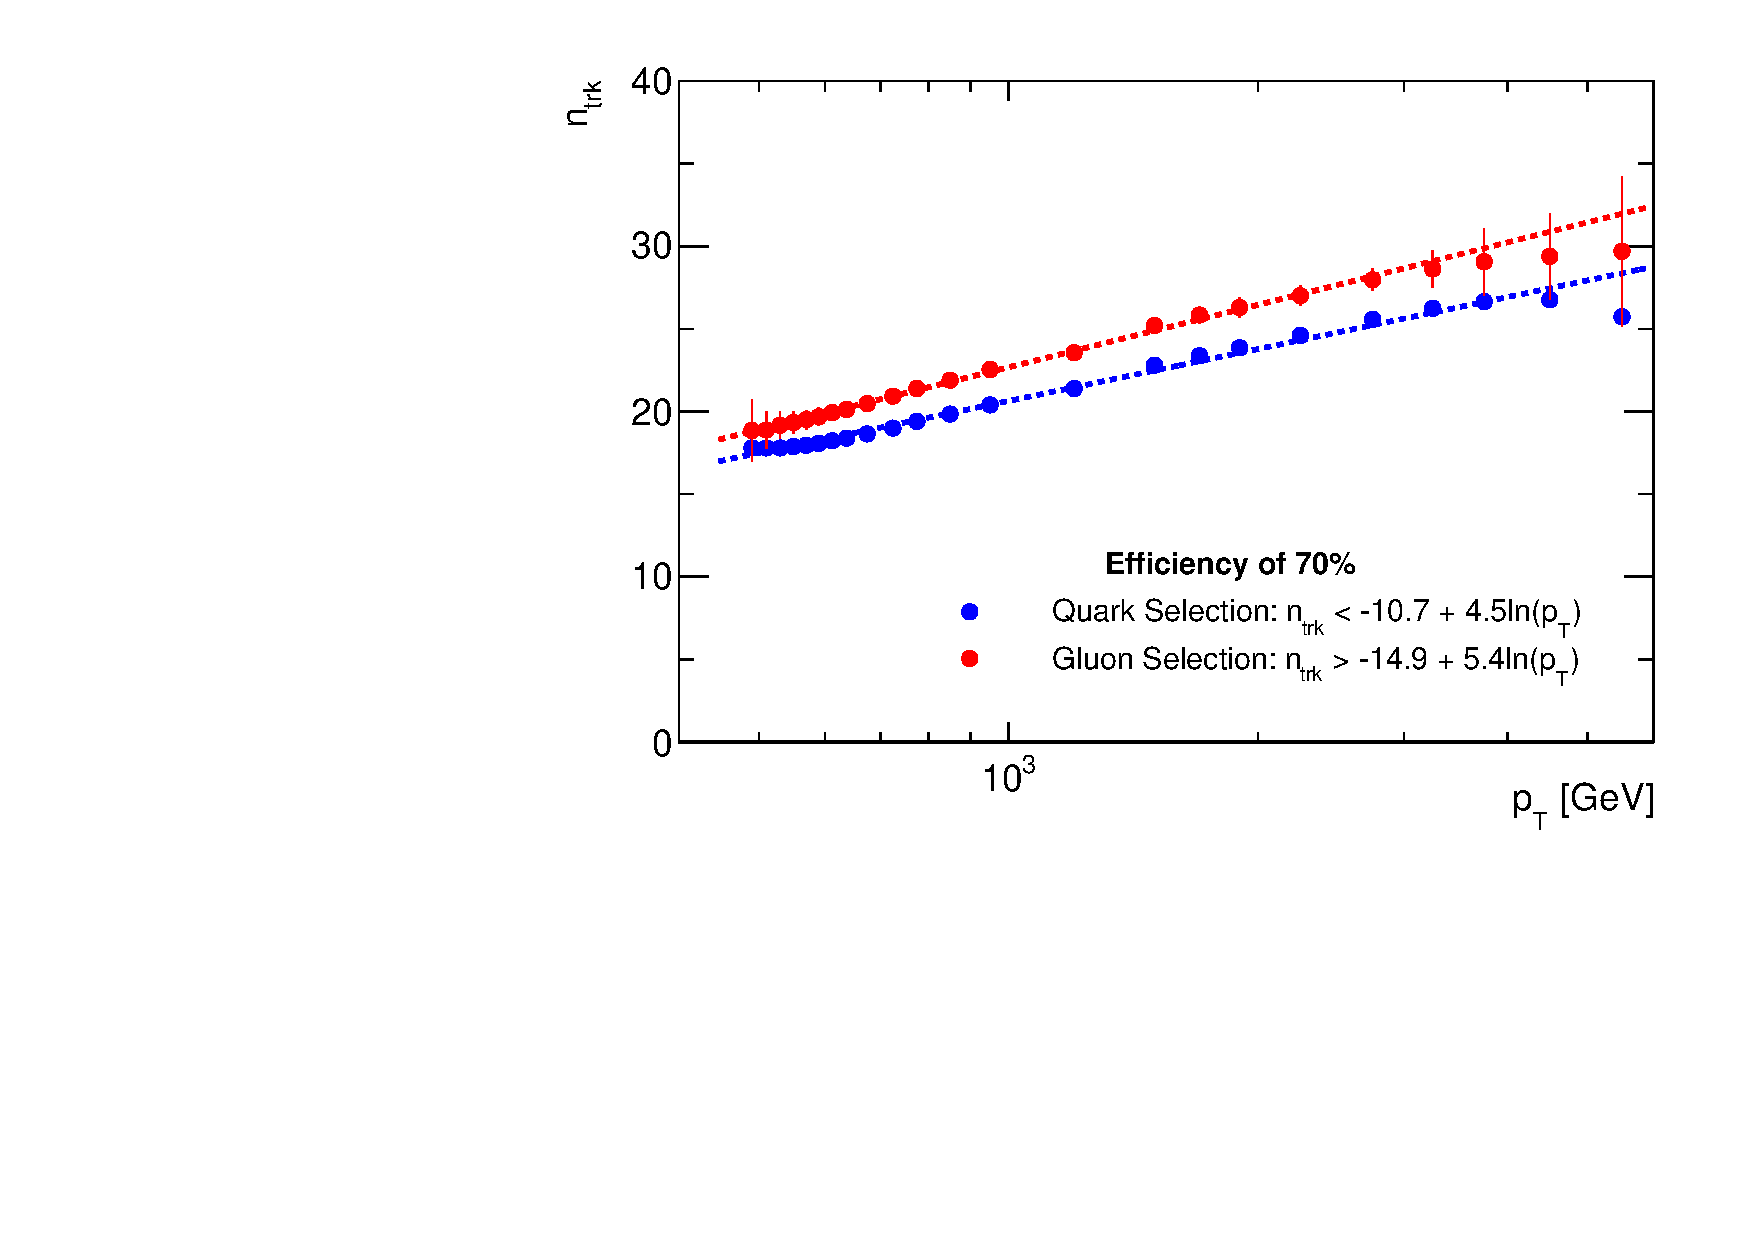
\includegraphics[width=0.45\textwidth]{fig/tagging_variation/quark_frac_selection_errors_6}}
	\subfloat[] {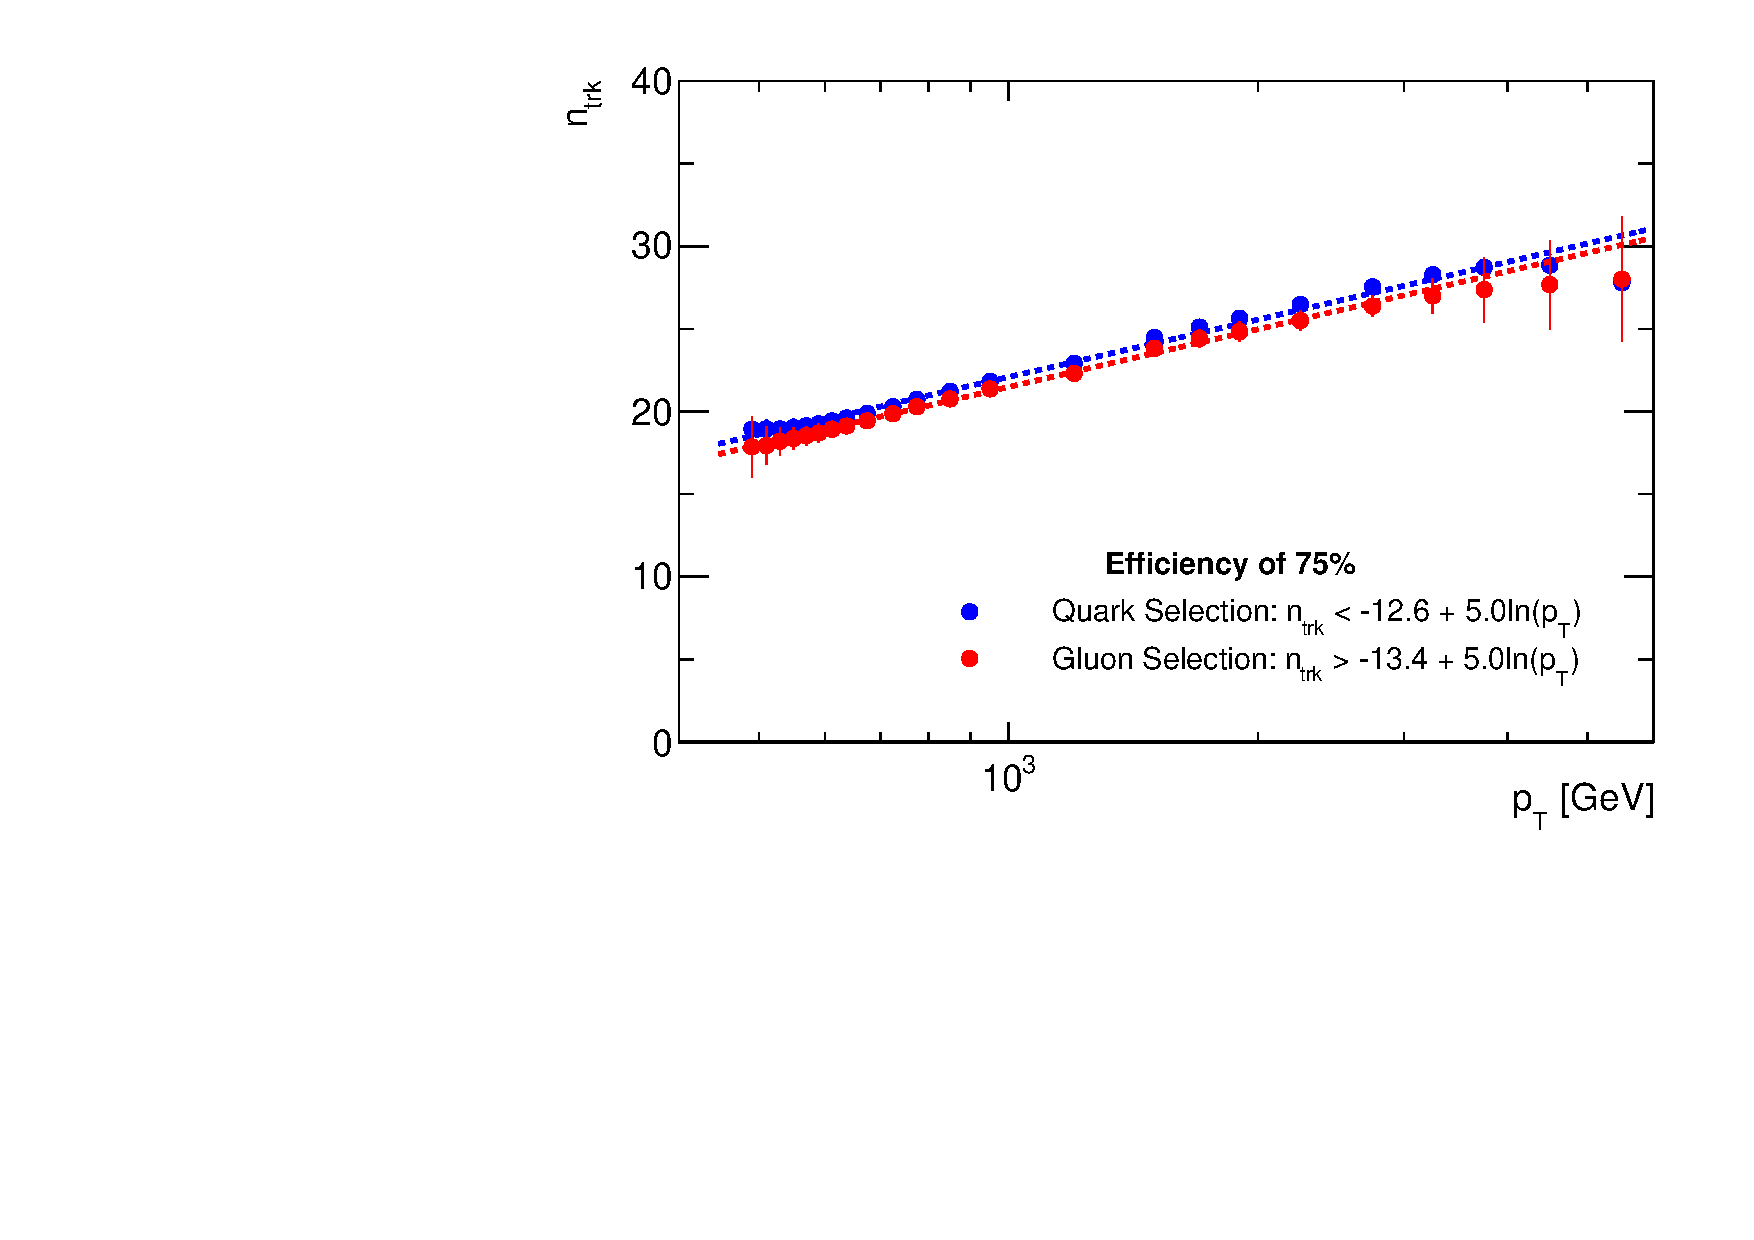
\includegraphics[width=0.45\textwidth]{fig/tagging_variation/quark_frac_selection_errors_5}}\\
	\subfloat[] {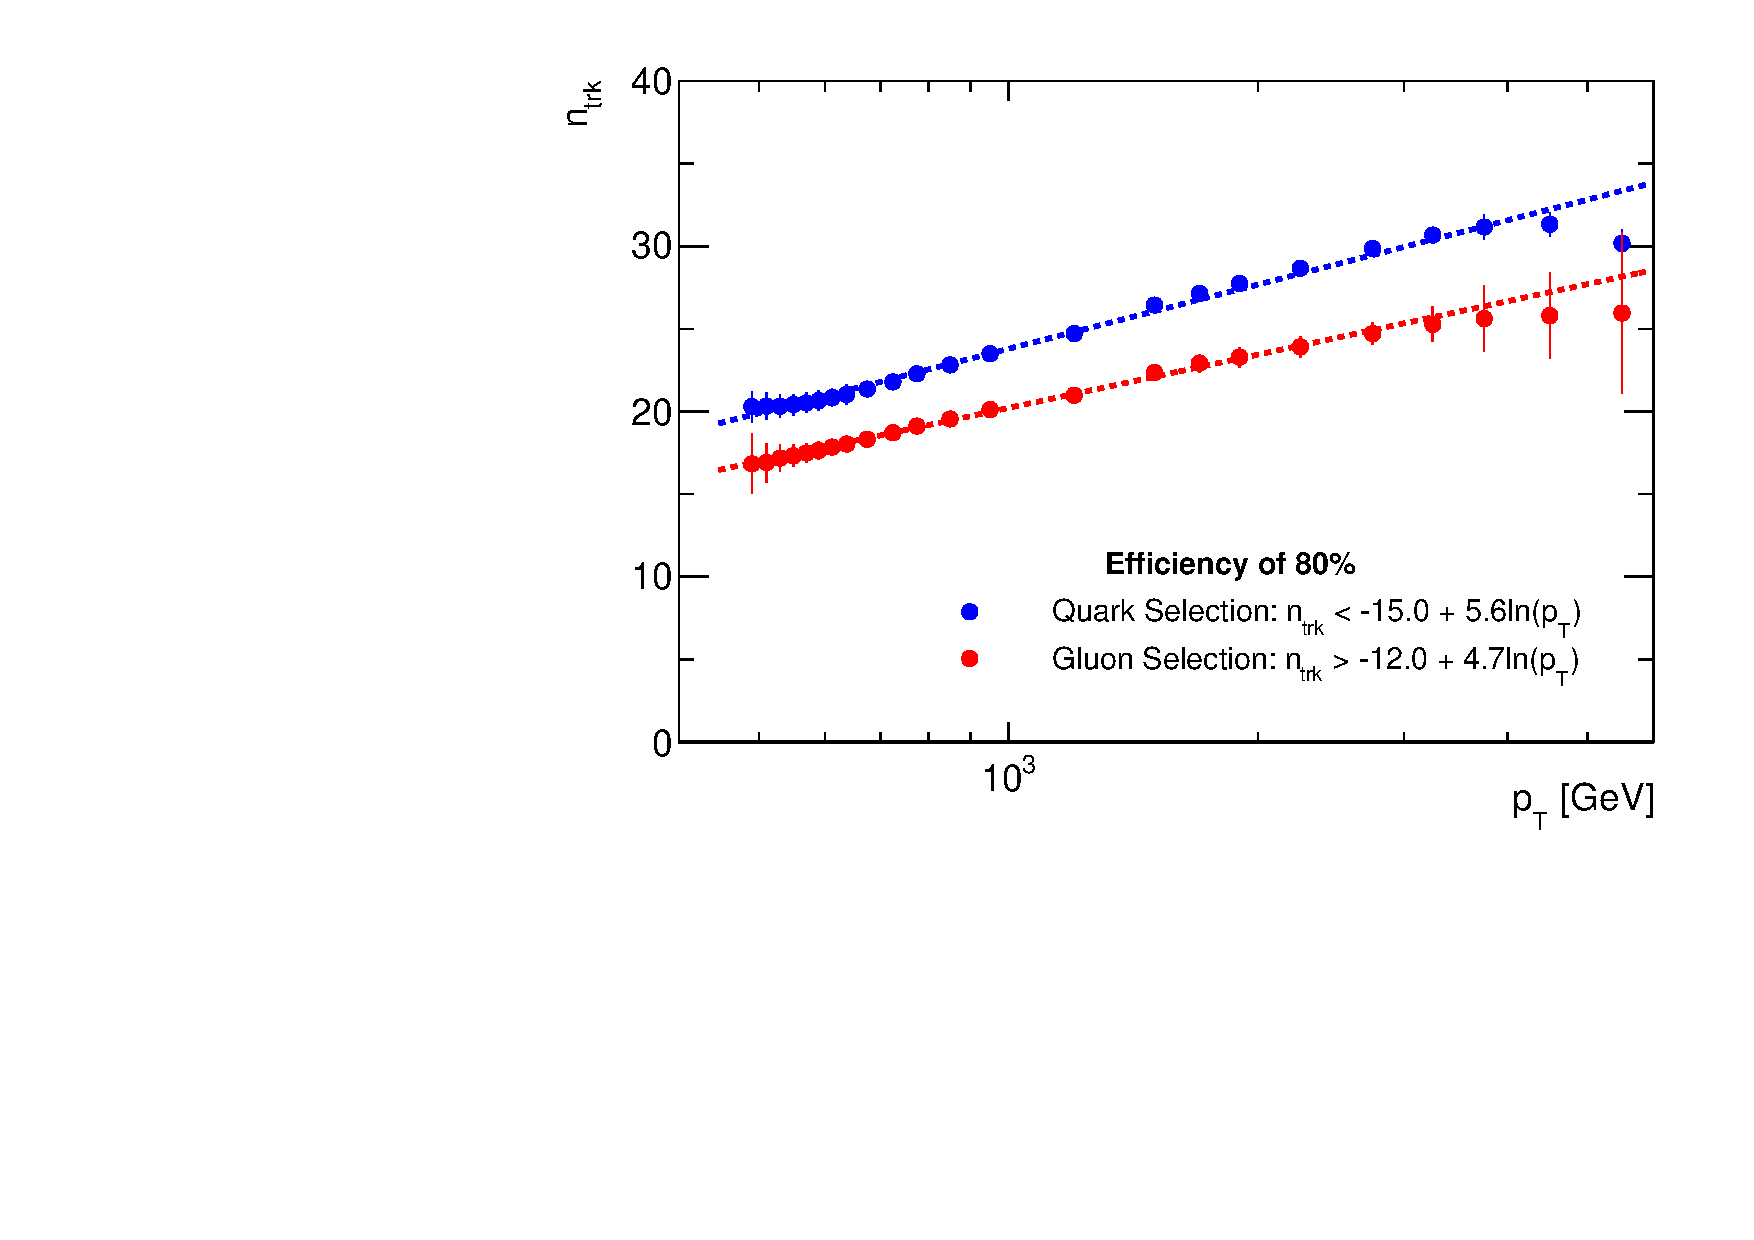
\includegraphics[width=0.45\textwidth]{fig/tagging_variation/quark_frac_selection_errors_4}}
	
	\caption{ The values of \ntrk\ for (a) 70\%,  (b) 75\%  and (c) 80\% quark (blue) and gluon (red) 
		selection efficiencies in each \pt\ bin along with the best fit to Equation~\ref{eq:nqg2}.
		\label{fig:qg_selection_curves_app}}
\end{figure}

\begin{figure}[p]
	\centering
	\subfloat[] {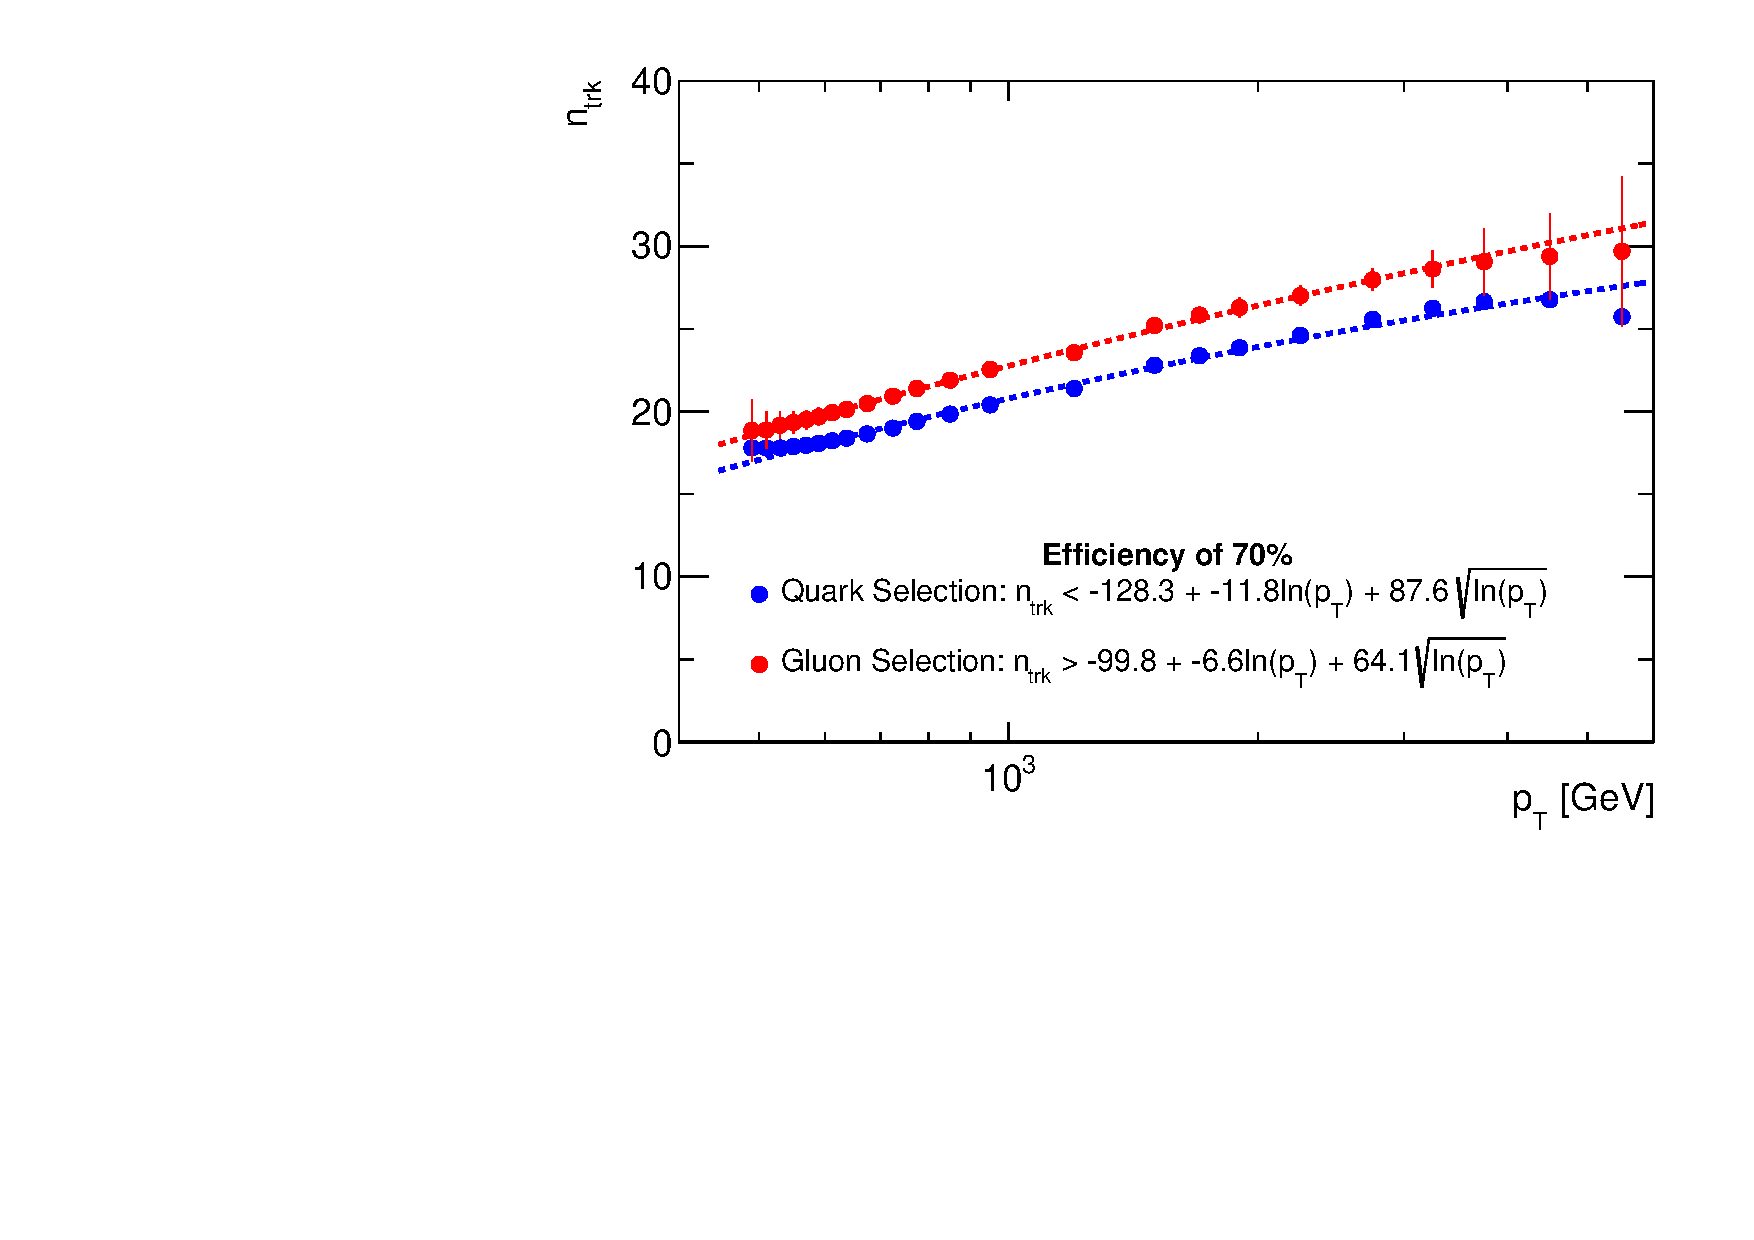
\includegraphics[width=0.45\textwidth]{fig/tagging_variation/quark_frac_newFit_selection_errors_6}}
	\subfloat[] {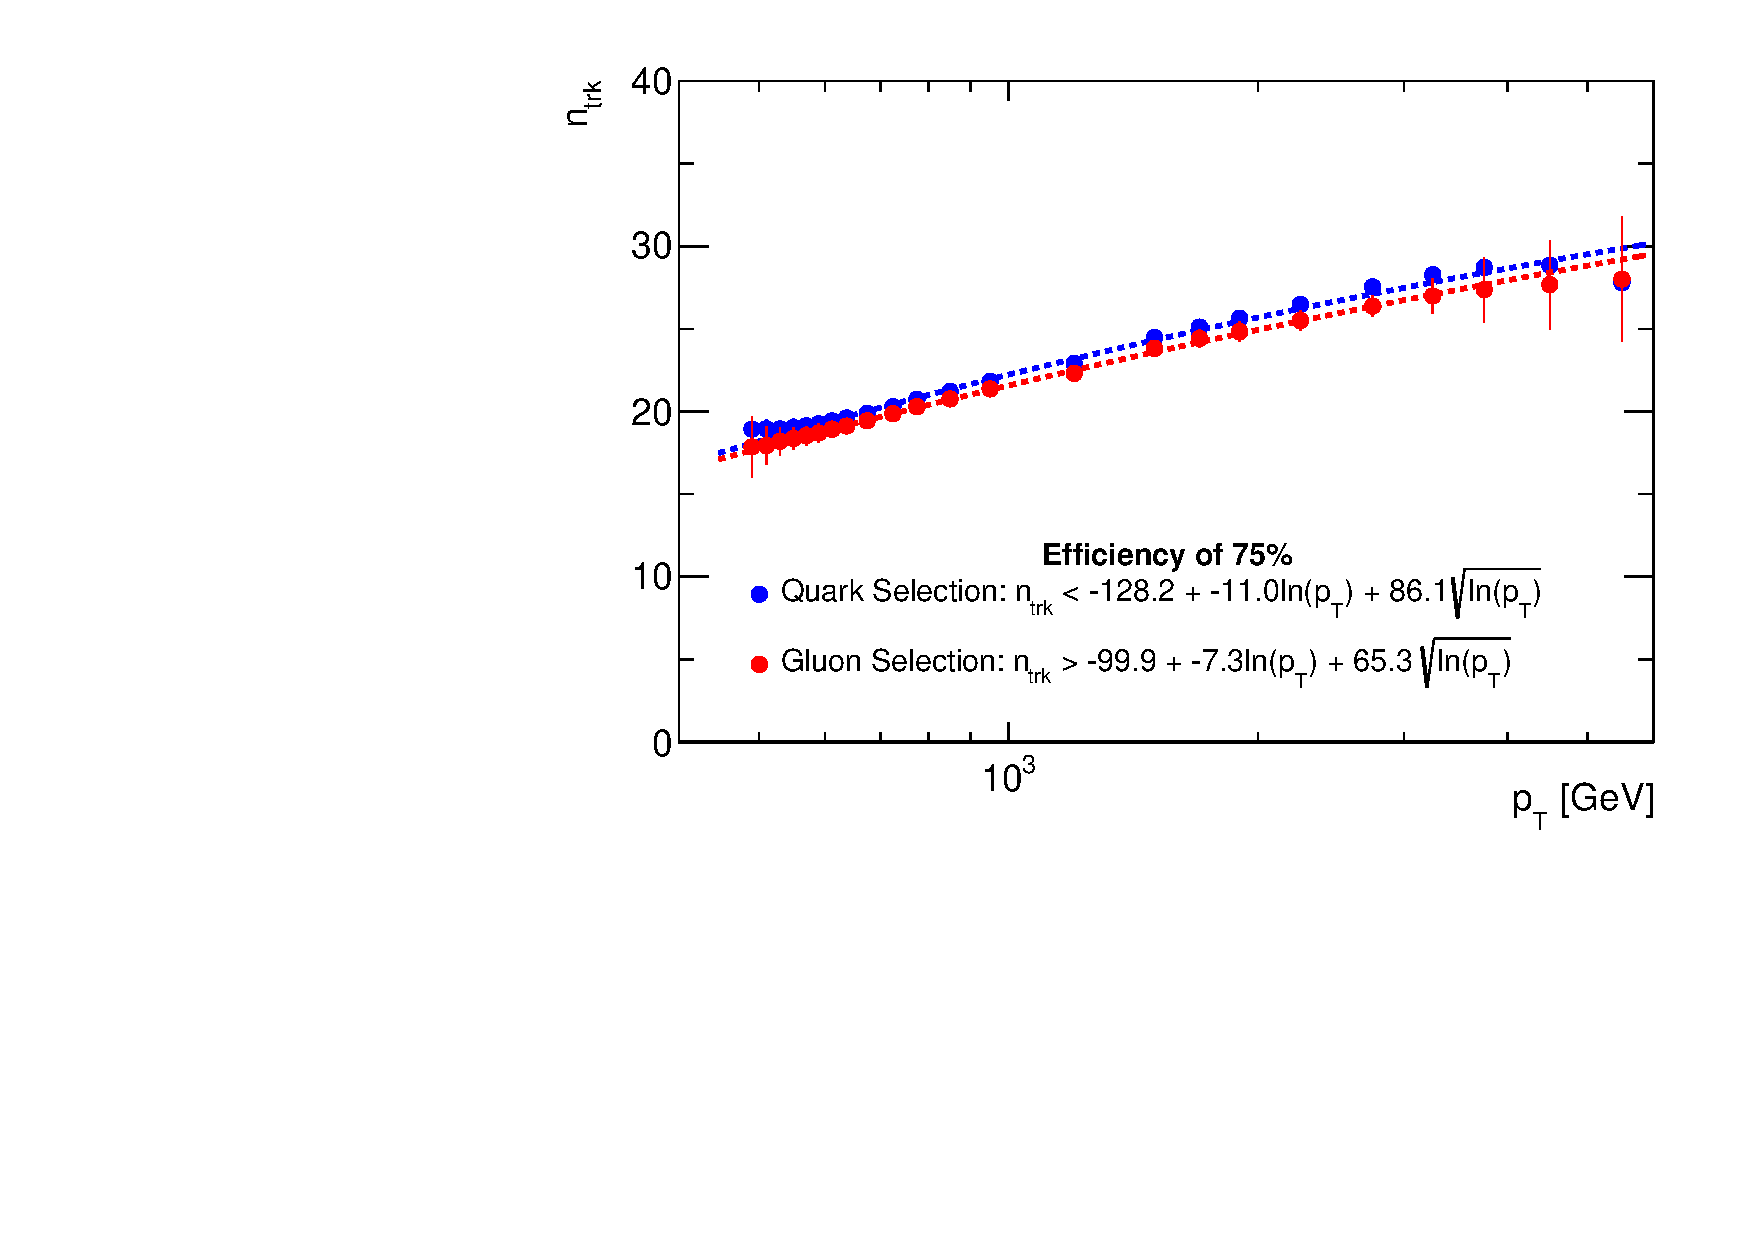
\includegraphics[width=0.45\textwidth]{fig/tagging_variation/quark_frac_newFit_selection_errors_5}}\\
	\subfloat[] {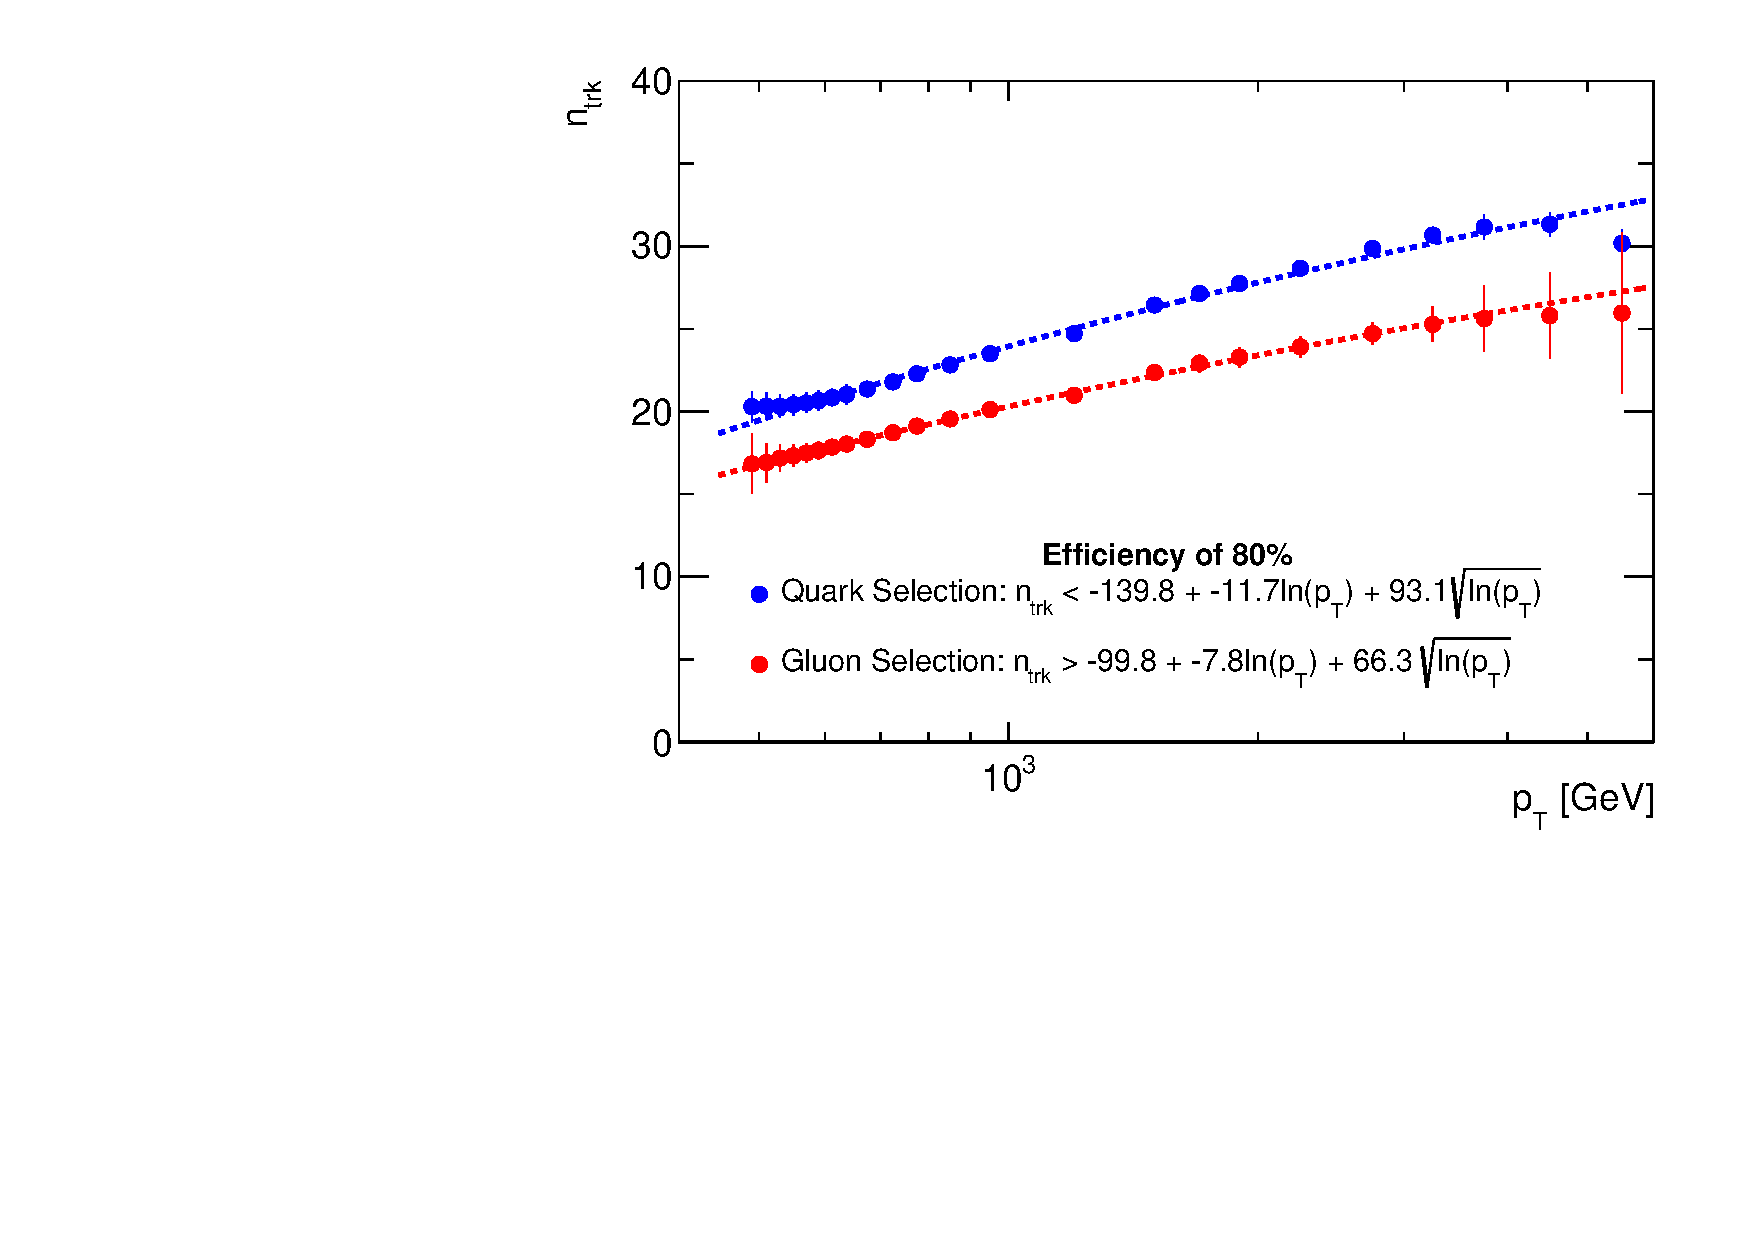
\includegraphics[width=0.45\textwidth]{fig/tagging_variation/quark_frac_newFit_selection_errors_4}}
	
	\caption{ The values of \ntrk\ for (a) 70\%,  (b) 75\%  and (c) 80\% quark (blue) and gluon (red) 
		selection efficiencies in each \pt~bin along with the best fit to Equation~\ref{eq:nqg3}.
		\label{fig:qg_selection_curves2}}
\end{figure}



\begin{table}[h]
	\centering 
	
	\begin{tabular}{SSSSS}
	\toprule
\multicolumn{1}{c}{Truth-$g$ selection efficiency}   & \multicolumn{1}{c}{Truth-$q$ selection efficiency} &  \multicolumn{1}{c}{$c$}  &  \multicolumn{1}{c}{$m$} &  \multicolumn{1}{c}{$n$}  \\
\midrule 
0.80 & 0.320 & -99.796 & -7.839 & 66.301 \\
0.75 & 0.274 & -99.949 & -7.271 & 65.347 \\
0.70 & 0.234 & -99.774 & -6.640 & 64.077 \\
\bottomrule
\end{tabular}
	\caption{ Values of constants $m$ and $c$ from Equation~\ref{eq:nqg3} such that $ \ntrk  \ge \ngluon $ 
	for truth quark jets for a range of efficiencies  from 70 to 80\%. 
	\label{table:truthGluonSelectionEfficiencies2}
}
\end{table}


\FloatBarrier


\paragraph{Signal Selection Efficiencies\\}

The \Hprime\ signal described in section~\ref{sec:hprime} is required to pass the selection criteria for a single jet gluon selection efficiency of 75\% given in Table~\ref{table:HprimeselctionEfficiency_app}. The selection efficiency for the \Hprime\ sample is expected to be 56.3\% ($0.75^2$ as both jets are required to be 75\%). In actual process, the ratio of \Hprime\ events that decay to two gluons ranges from 51.9\% for a 2 TeV signal to 57.4\% for a 7 TeV signal.

The effective fraction of \Hprime\ events decaying into two gluons is slightly below 100\%, due to factors like gluon splitting and other showering effects. This fraction varies from 91.3\% to 95.4\%. The discrepancy between the actual efficiency and the expected efficiency (56.3\% of the truth efficiency) is depicted in Figure~\ref{fig:HPrime_efficiency_difference}. The average difference across selection criteria is approximately 3.3\%.

Since there is minimal distinction between the two selection criteria, the simpler choice outlined in Equation~\ref{eq:nqg2} will be adopted.

\begin{table}[h]
	\centering 
	\begin{tabular}{SSSS}
	\toprule
\multicolumn{1}{c}{\Hprime\ Mass (GeV)}   & \multicolumn{3}{c}{Selection efficiency(\%)} \\
\multicolumn{1}{c}{} & \multicolumn{1}{c}{Equation~\ref{eq:nqg2}} & \multicolumn{1}{c}{Equation.~\ref{eq:nqg3} ($\sqrt{}$ term)} 
& \multicolumn{1}{c}{Truth} \\
\midrule 
2000	&	51.9 & 51.8& 91.3 \\
2500	&	53.2 & 53.0& 91.7 \\
3000 	&	54.9 & 54.6& 92.3 \\
3500	&	55.3 & 55.1& 93.4 \\
4000	&	56.4 & 56.2& 93.4 \\
4500	&	56.7 & 56.7& 94.1 \\
5000	&	56.2 & 56.4& 94.3 \\
5500	&	57.2 & 57.5& 94.9 \\
6000	&	57.4 & 57.8& 95.1 \\
6500	&	57.4 & 58.3& 95.5 \\
7000	&	57.4 & 58.1& 95.4 \\\bottomrule
\end{tabular}
	\caption{ The signal selection efficiency for a fully simulated \Hprime\ decaying to two gluons with requiring two jets to 
	pass the 75\% single jet criteria given in Equation~\ref{eq:nqg2} with constants from 
	Table~\ref{table:truthGluonSelectionEfficiencies_app} and the criteria given in Equation~\ref{eq:nqg3} with constants from 
	Table~\ref{table:truthGluonSelectionEfficiencies2}.  
	The expected double tagged gluon efficiency is 56.3\%. 
	\label{table:HprimeselctionEfficiency_app}
}
\end{table}


\begin{figure}[p]
 \centering
 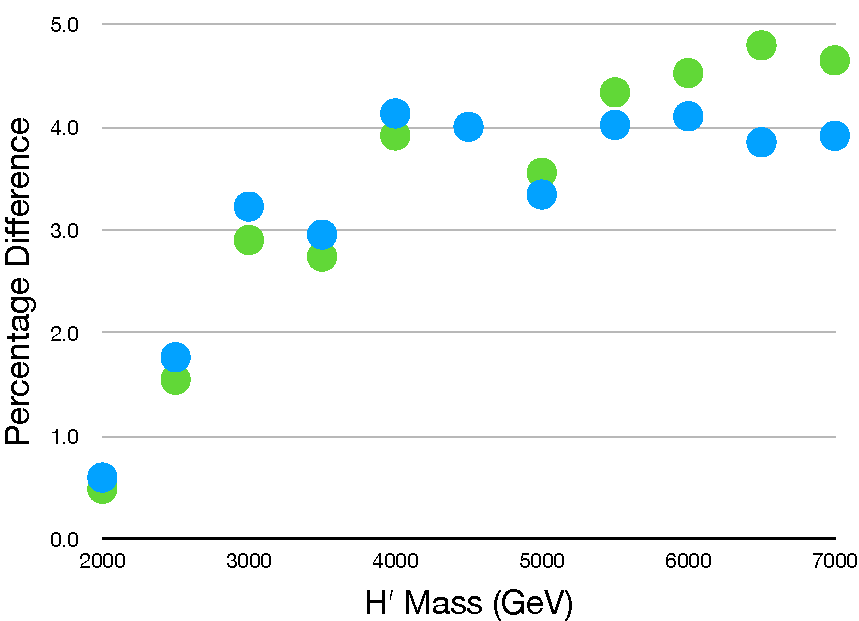
\includegraphics[width=0.60\textwidth]{fig/tagging_variation/HPrime_Efficiency_Difference}
\caption{ The difference between the expected signal selection efficiency of 56.3\%
for a single jet selection efficiency of 75\% for \Hprime\ using Equation~\ref{eq:nqg2} (Blue) and
Equation~\ref{eq:nqg3} (Green)}
 \label{fig:HPrime_efficiency_difference}}
\end{figure}




%The constants $m$ and $c$ are found by finding the value of \ntrk\ 
%that corresponds to a given efficiency for truth quark and gluon jets in 
%\pT\ bins and fitting the results. For each \pT\ bin the number of tracks 
%closest to the chosen selection efficiency is found. Since this is an integer 
%number of tracks and does and does not correspond exactly to the selection efficiency 
%a correction is applied by estimating the fractional number of tracks that corresponds 
%to the selection  efficiency  by carrying out a linear interpolation between the efficiencies 
%for the selected bin and its nearest neighbour. The uncertainty on this value is then estimated using 
%binomial uncertainties. 



%The constants $m_{\mathrm{q(g)}}$ and $c_{\mathrm{q(g)}}$ are found by finding the value of \ntrk\ 
%that corresponds to a given efficiency for truth quark and gluon jets in 
%\pT\ bins and fitting the results to Eq.~\ref{eq:nqg2}.  The jet \pT\ bin edges are chosen to be 
%400, 500, 650, 800, 1000, 1200, 1500, 2000, 3000, 6000\,\GeV. An example of the \ntrk cumulative 
%distribution for truth quark and gluon jets satisfying $800 < \pT < 1000\,\GeV$ is shown in
%Fig.~\ref{fig:ntrk_cumulative}.
%
%
%
%%The jet \pT\ bin edges are chosen to be 
%%480, 500, 520, 540, 560, 580, 600, 625, 650, 700, 750, 800, 900, 1000, 1400, 
%%1600, 1800, 2000, 2500, 3000, 3500, 4000, 5000, 6000\,\GeV. An example of the \ntrk cumulative 
%%distribution for truth quark and gluon jets satisfying $800 < \pT < 900\,\GeV$ is shown in
%%Fig.~\ref{fig:ntrk_cumulative}.
%
%
%%\begin{figure}[htb]
%% \centering
%%\includegraphics[width=0.75\textwidth]{figures/tagging/Cumulative_ntrk_distribution_12_800_900GeV.pdf}
%%\caption{The cumulative distribution of \ntrk\ for truth quark (blue) and gluon (red) initiated jets 
%%satisfying $800 < \pT < 900\,\GeV$.  \label{fig:ntrk_cumulative}}
%%\end{figure}
%
%\begin{figure}[htb]
% \centering
%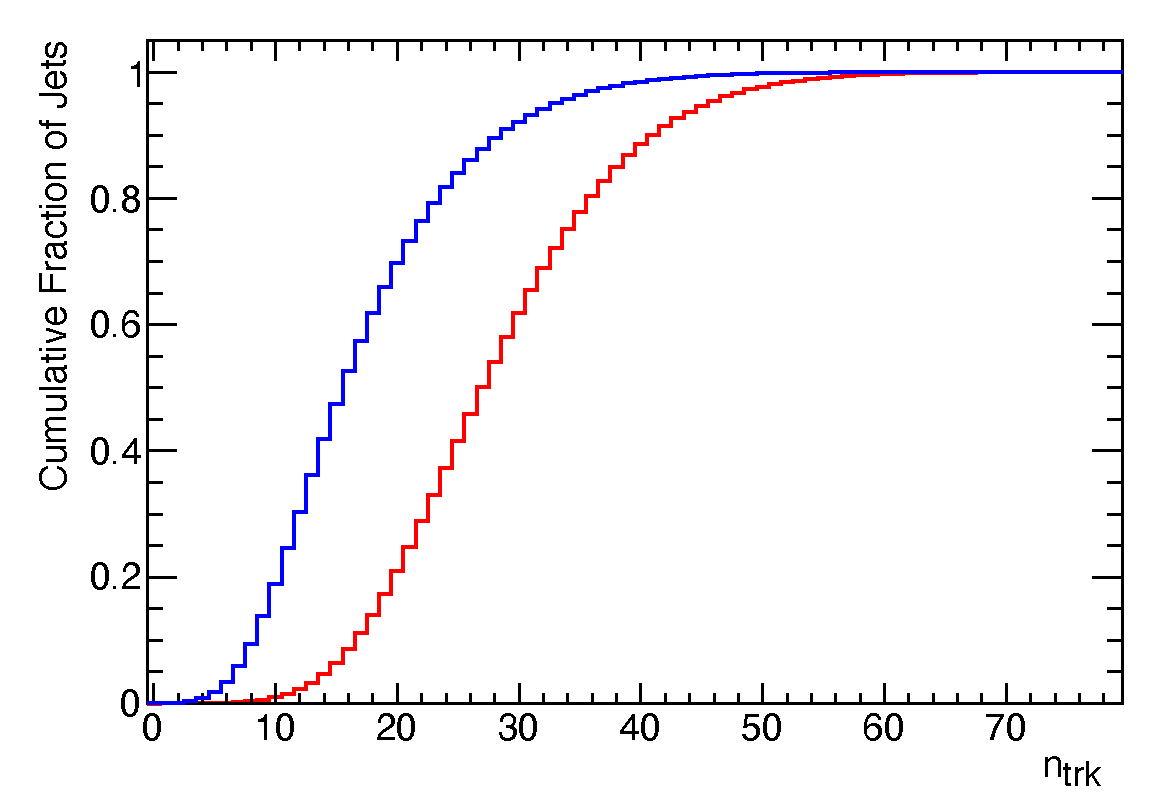
\includegraphics[width=0.75\textwidth]{figures/tagging/Cumulative_ntrk_distribution_4_800_1000GeV.pdf}
%\caption{The cumulative distribution of \ntrk\ for truth quark (blue) and gluon (red) initiated jets 
%satisfying $800 < \pT < 1000\,\GeV$.  \label{fig:ntrk_cumulative}}
%\end{figure}
%
%
%The constants for Eq.~\ref{eq:nqg2} are found for quark and gluon selection efficiencies from 
%65\% to 95\% in 5\% steps. The plot of the value of \ntrk\ that satisfies the selection efficiencies 
%of 70 and 80\% are shown in Fig.~\ref{fig:qg_selection_curves} along with the best fit using Eq.~\ref{eq:nqg2}.
%The values of the constants for both quark and gluon selections are summarised in 
%Tables~\ref{table:truthQuarkSelectionEfficiencies} and \ref{table:truthGluonSelectionEfficiencies}.
%
%\begin{figure}[htb]
% \centering
%  \subfigure[] {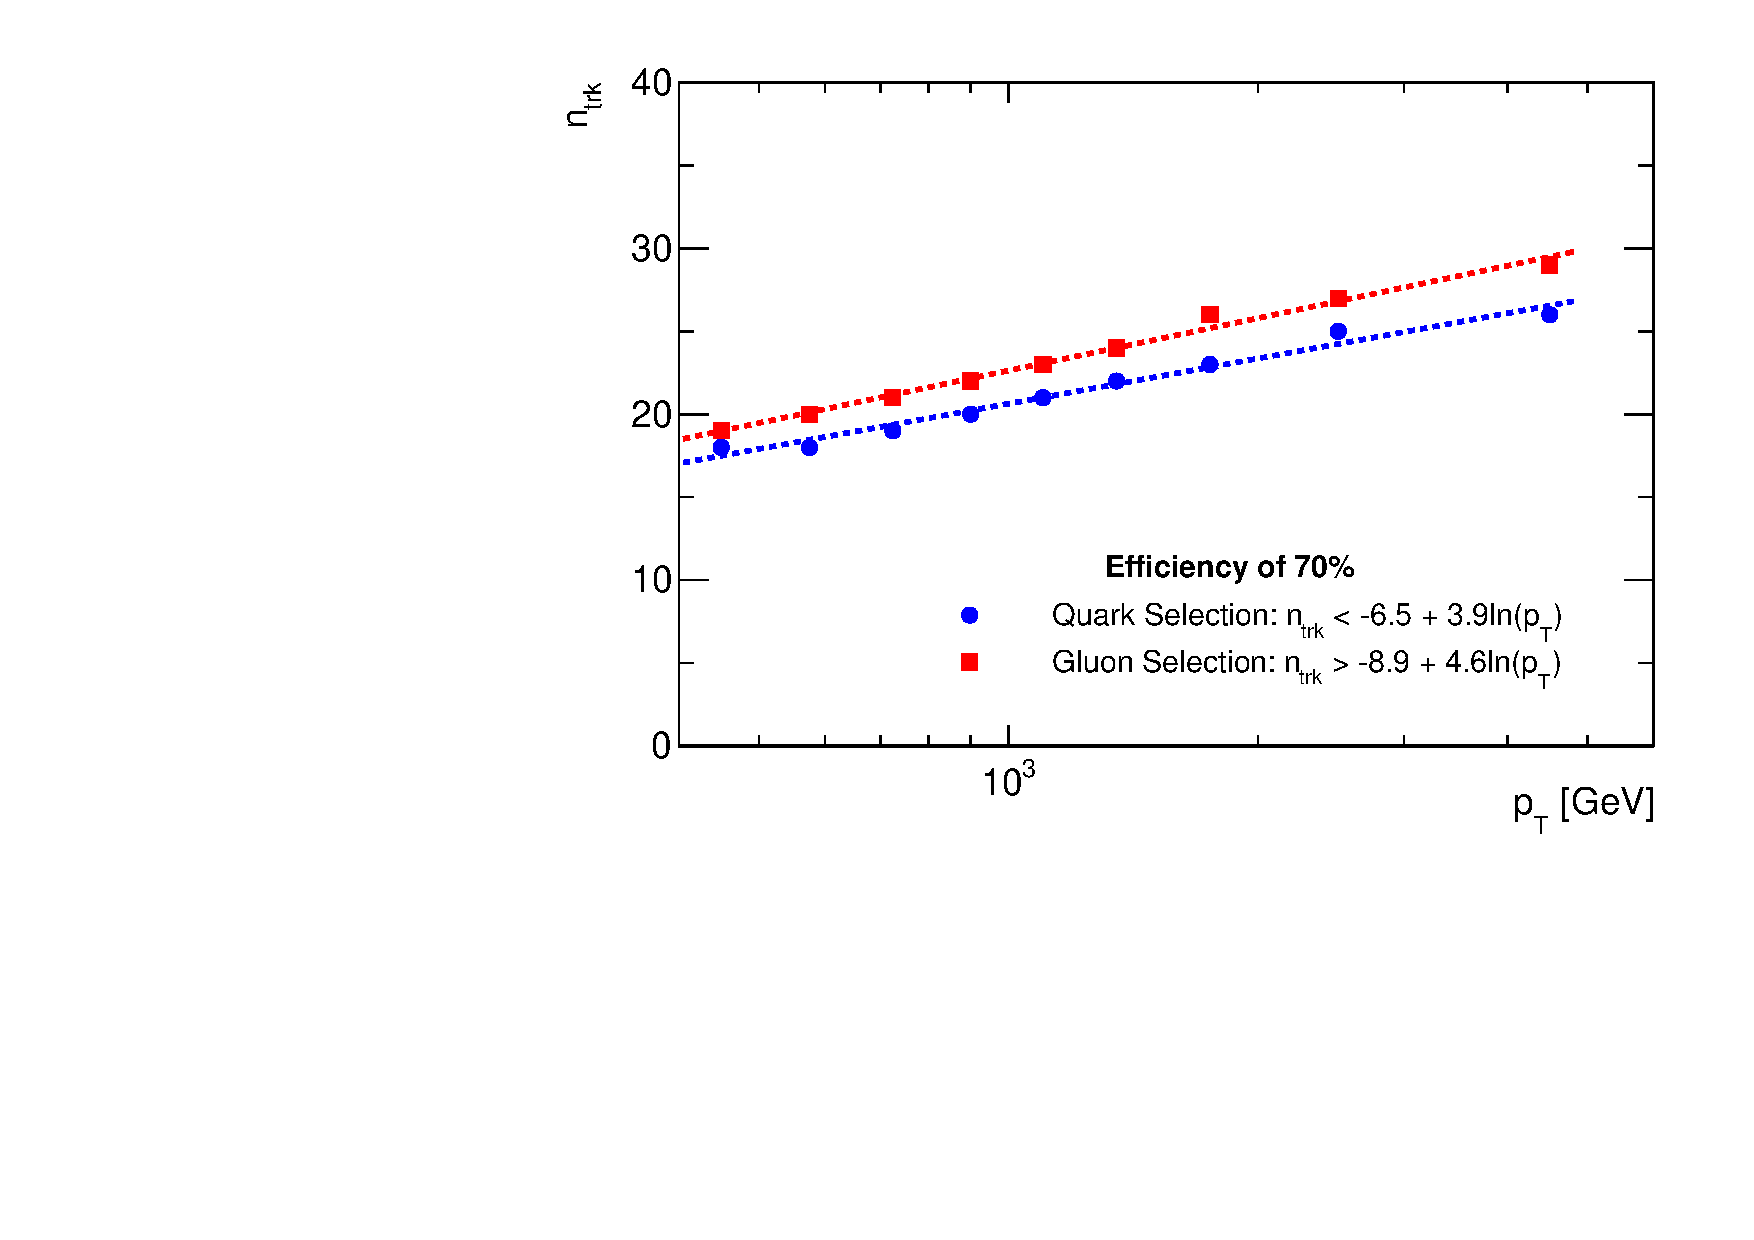
\includegraphics[width=0.495\textwidth]{figures/tagging/quark_selection_6}}
%  \subfigure[] {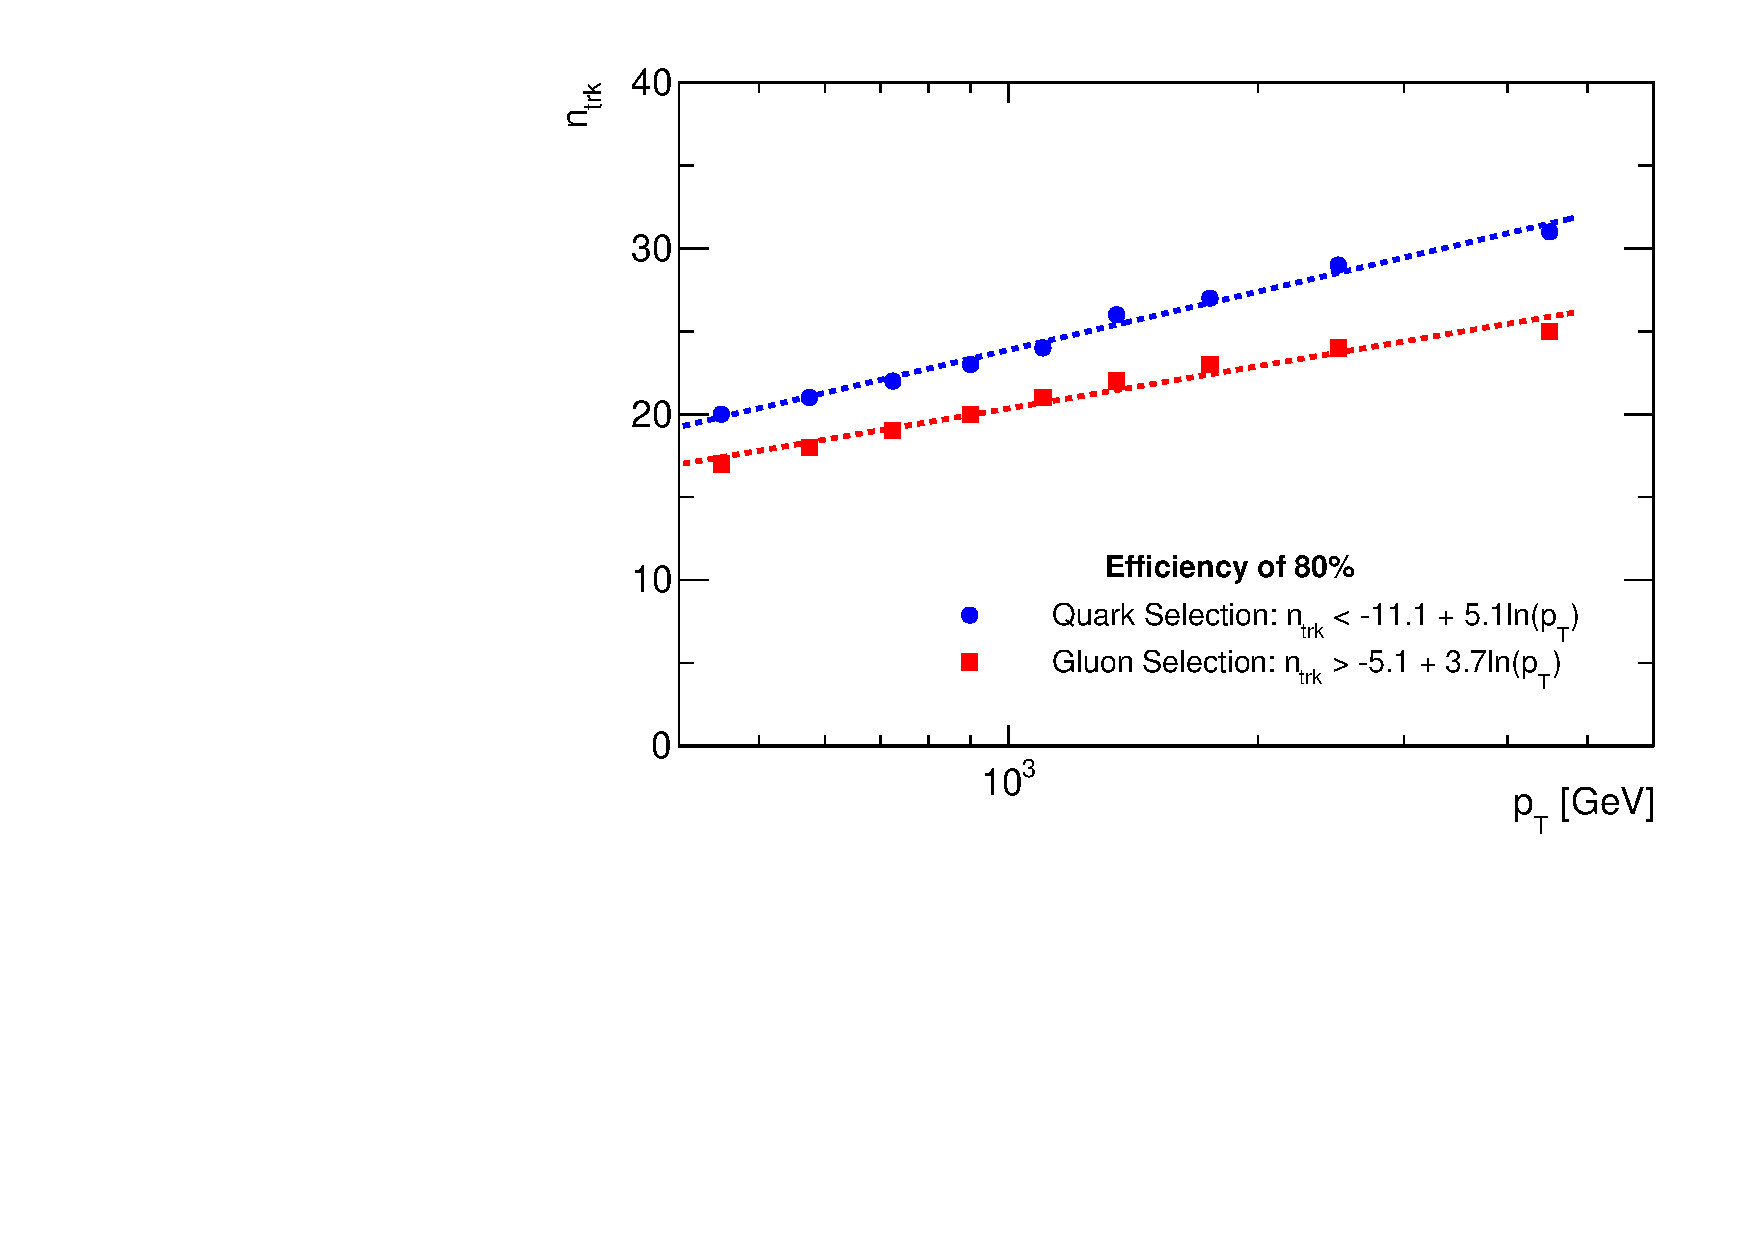
\includegraphics[width=0.495\textwidth]{figures/tagging/quark_selection_4}}
%
%\caption{ The values of \ntrk\ for (a) 70\% and (b) 80\% quark (blue) and gluon (red) 
%selection efficiencies in each \pT\ bin along with the best fit to Eq.~\ref{eq:nqg2}.
% \label{fig:qg_selection_curves}}
%\end{figure}
%
%
%\begin{table}[h]
%	\centering 
%		\caption{ Values of constants $m$ and $c$ from Eq.~\ref{eq:nqg2} such that $ \ntrk  \le \nq $ 
%		for truth quark jets for a range of efficiencies  from 65 to 95\%. 
%		\label{table:truthQuarkSelectionEfficiencies}
%		}
%	\begin{tabular}{SSSS}
%	\toprule
%\multicolumn{1}{c}{Truth-$q$ selection efficiency}   & \multicolumn{1}{c}{Truth-$g$ selection efficiency} &  \multicolumn{1}{c}{$c_{\mathrm{q}}$}  &  \multicolumn{1}{c}{$m_{\mathrm{q}}$} \\
%\midrule 
%0.95 & 0.73 & -20.0 & 7.7 \\
%0.90 & 0.57 & -15.9 & 6.5 \\
%0.85 & 0.45 & -13.1 & 5.6 \\
%0.80 & 0.36 & -11.1 & 5.1 \\
%0.75 & 0.28 & -9.1  & 4.5 \\
%0.70 & 0.22 & -6.5  & 3.9 \\
%0.65 & 0.18 & -4.4  & 3.5 \\
%\bottomrule
%\end{tabular}
%\end{table}
%
%\begin{table}[h]
%	\centering 
%		\caption{ Values of constants $m$ and $c$ from Eq.~\ref{eq:nqg2} such that $ \ntrk  \ge \ngluon $ 
%		for truth gluon jets for a range of efficiencies  from 65 to 95\%. 
%		\label{table:truthGluonSelectionEfficiencies}
%		}
%	\begin{tabular}{SSSS}
%	\toprule
%\multicolumn{1}{c}{Truth-$g$ selection efficiency}   & \multicolumn{1}{c}{Truth-$q$ selection efficiency} &  \multicolumn{1}{c}{$c_{\mathrm{g}}$}  &  \multicolumn{1}{c}{$m_{\mathrm{g}}$} \\
%\midrule 
%0.95 & 0.59 & -3.9 & 2.7 \\
%0.90 & 0.46 & -4.3 & 3.1 \\
%0.85 & 0.39 & -5.4 & 3.5 \\
%0.80 & 0.31 & -5.1 & 3.7 \\
%0.75 & 0.27 & -7.3 & 4.2 \\
%0.70 & 0.23 & -8.9 & 4.6 \\
%0.65 & 0.20 & -8.0 & 4.6\\
%\bottomrule
%\end{tabular}
%\end{table}
%
%
%\subsubsection{Signal Selection Efficiencies}
%
%
%The selection criteria for a single jet gluon selection efficiency of 75\% is applied to the \Hprime\ 
%sample described in in section~\ref{sec:hprime} are given in Table~\ref{table:HprimeselctionEfficiency}. 
%If the selection works perfectly the expected selection efficiency for the \Hprime\ sample would be 56.3\% ($0.75^2$). 
%The actual selection efficiencies range between 51.9\% for a 2\,\TeV\ signal to 57.4\% for a 7\,\TeV\ signal. 
%
%The actual fraction of \Hprime\ events that decay to two gluons is less than 100\% due to gluon splitting and other showering 
%effects and ranges from 91.3 to 95.4\%. The variation between the expected efficiency (56.3\% of the truth efficiency) 
%is plotted in Fig.~\ref{fig:HPrime_efficiency_difference}. The average difference for is approximately 3.3\% for both selection criteria.
%
%%There is negligible difference between the two selection criteria so the simpler choice as given in Eq.~\ref{eq:nqg2} will be used.
%
%
%
%\begin{table}[h]
%	\centering 
%		\caption{ The signal selection efficiency for a fully simulated \Hprime\ decaying to two gluons with requiring two jets to 
%		pass the 75\% single jet criteria given in Eq.~\ref{eq:nqg2} with constants from 
%		Table~\ref{table:truthGluonSelectionEfficiencies} and the criteria given in Eq.~\ref{eq:nqg3} with constants from 
%		Table~\ref{table:truthGluonSelectionEfficiencies2}.  
%		The expected double tagged gluon efficiency is 56.3\%. 
%		\label{table:HprimeselctionEfficiency}
%		}
%	\begin{tabular}{SSS}
%	\toprule
%\multicolumn{1}{c}{\Hprime\ Mass (\GeV)}   & \multicolumn{2}{c}{Selection efficiency(\%)} \\
%\multicolumn{1}{c}{} & \multicolumn{1}{c}{Eq.~\ref{eq:nqg2}} &  \multicolumn{1}{c}{Truth} \\
%\midrule 
%2000	&	51.9 & 91.3 \\
%2500	&	53.2 & 91.7 \\
%3000 	&	54.9 & 92.3 \\
%3500	&	55.3 & 93.4 \\
%4000	&	56.4 & 93.4 \\
%4500	&	56.7 & 94.1 \\
%5000	&	56.2 & 94.3 \\
%5500	&	57.2 & 94.9 \\
%6000	&	57.4 & 95.1 \\
%6500	&	57.4 & 95.5 \\
%7000	&	57.4 & 95.4 \\\bottomrule
%\end{tabular}
%\end{table}
%
%
%\clearpage
%
